\chapter{Le mouvement réformiste (fin XIXe - début XXe)}
  \mn{(07/02/2022)}
 
 
  
  `ABDUH Muhammad, \emph{Rissalat ai Tawhid - Exposé de la religion
  musulmane}, Geuthner, Paris, 1925, trad. fr. et introduction B. Michel
  et Ch. Moustapha Abdel Razik.
  
 
  
  AL-AFGHANI Jamâl ad-Din, \emph{La réfutation des matérialistes},
  Geuthner, Paris, 1942, trad. fr. A.-M. Goichon. Textes divers in:
  \emph{Orient}, 1962, N° 21 p. 89-115, N°22 p. 125-160, N° 23 p. 169-
  198, N' 24 p. 125-152 et \emph{Orient}, 1963, N° 25 p. 141-152.
 


HADDAD, Mohammed \emph{Le réformisme musulman : une histoire critique},
Paris, Mimesis, 2013. HOURANI, Albert \emph{La pensée arabe et
l'Occident,} Groupe Naufal Europe, Paris, 1991.

JOMIER Jacques \emph{Le Commentaire coranique du Manâr}, Maisonneuve,
Paris, 1954.

MERAD Ali \emph{Le réformisme musulman en Algérie de 1925 à 1940. Essai
d'histoire religieuse et sociale}, Paris, Mouton et Cie, 1967.
 \emph{Ibn Bâdis,
commentateur du Coran}, Geuthner, Paris, 1971.

METCALF, Barbara \emph{Islamic Revival in British India 1860-1900},
Princeton University Press, 1982.

TROLL, Christian \emph{Sayyid Ahmad Khân. A Reinterpretation of Muslim
Theology}, Vikas Publ.

House, New Delhi, 1978.



 \section{Introduction : Arrière fond positiviste}
 
 \paragraph{Auguste Comte}
 
 \paragraph{idée de progrès} Évolutionnisme de société. Le progrès est porté par l'occident. Vision des sociétés évoluant vers un mieux, du coup, hiérarchisation des sociétés, entre les sociétés archaïques et celles qui s'appuient sur la Raison et ont dépassé le stade de la religion.
 
 \paragraph{Acceptation des valeurs occidentales} souveraineté du peuple; droits individuels; liberté d'expression. 
 
 \paragraph{Un discours critique de la Religion} 
 
  %-----------------------------------------------------------------------------------
  \section{Les « Occidentalisants »}
  
\paragraph{trois premiers quarts du XIX} jeunes de l'élite de l'empire Ottoman. L'empire cherche à se réformer en introduisant des éléments européeans. L'Empire Ottoman envoie des jeunes en France pour se former.

\paragraph{Tahtawi} Egyptien, a vécu 5 ans en France (1826-1831). A été ensuite dans l'administration ottomane. \textit{L'Or de Paris}\sn{très intéressant à lire}

\paragraph{Khayr ad-din} Caucasien, installé en Tunisie. A vécu à Paris (1852-1856).

\paragraph{Jeunes ottomans} dans le contexte turque. 

\paragraph{Ils notent le désir de progrès} A la différence de Al Wahhab qui est soupçonneux de l'\textit{innovation}, on valorise le changement social : 
\begin{quote}
    quiconque maitrise un art désire inventer quelque chose inconnu auparavant \sn{Or de Paris}
\end{quote}

 
 \paragraph{État}  Sur le plan politique, une compréhension différente de l'État. Dans le cadre classique, l'État doit assurer la justice. Or, ici l'État encadre le progrès de la société. Ils sont convaincus que ce sont les institutions politiques qui sont à l'origine de la force des États occidentaux. Par contre, ils vont être en retrait sur l'approche critique de la religion du positivisme.
 
 \paragraph{les lumières ont émancipé l'Europe de l'obscurantisme chrétien} avec une pointe polémique : les lumières viennent de la philosophie musulmane, et donc adopter les lumières pour les musulmans, ce n'est pas trahir le patrimoine musulman, c'est se le réapproprier. \sn{C'est la pointe de Tariq Ramadan dans les années 1990}.
 
 \paragraph{Principes politiques} Ils vont associer les principes démocratiques au principe de la \emph{Shura}, \textit{consultation}, principe coranique de consultation des notables, reinterprété dans un contexte moderne.
 \begin{Def}[shura]
    \emph{ intention} - consultation
\end{Def} 
 \paragraph{droit musulman} dans un cadre musulman, Il faut moderniser le droit musulman pour qu'il puisse accompagner le développement de la société. Ils pronent une unification du droit, une seule école, moderne et uniforme. Il faut viser à l'éducation des jurisconsultes, dans un cadre moderne. 
  
  %-----------------------------------------------------------------------------------
  \section{Trois grands réformistes}
   
   Après les occidentalisants, qui préfigurent les modernistes, il y a les réformistes que l'on verra à travers trois figures.
   
   \paragraph{Seyyed Ahmad Khan (1817-1898)} Il ne sort pas de nul part, son père est soufi et sa mère a été formé dans une école fondé par Walî Allâh (P \pageref{Theo:waliAllah}). Très grande figure en Inde
   
   \paragraph{Jamal ad-din Al Afghani (1839-1897)} formé en Inde mais action dans l'Empire Ottoman (séjour important en Egypte (1871-79)) et un autre à Paris où il est exilé (1881-1883). C'est un activiste  : revues, société secrète. Son but est de lutter contre la colonisation. Il finit sa vie sous surveillance ottomane.
   
   \begin{figure}
       \centering
       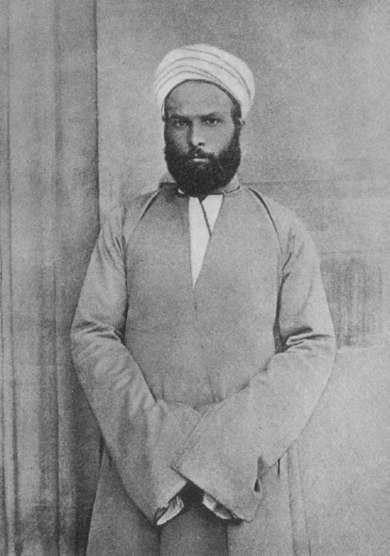
\includegraphics{390px-Muhammad_Abduh}
       \caption{Caption}
       \label{fig:my_label}
   \end{figure}
   \mn{\href{Mohamed Abduh}{https://fr.wikipedia.org/wiki/Mohamed_Abduh}
   }
    \paragraph{Muhammad Abduh} Egyptien, successeur d'Al Afghani. Il a ensuite développé sa propre pensée. Surtout en Egypte mais a partagé le séjour parisien de \textit{Aghani} puis au Liban. On lui a interdit d'enseigner mais il a été nommé grand mufti d'Egypte (1899). On avait moins peur de son activité du droit que de son activité sur les jeunes en tant qu'enseignant. Fonde aussi une école qui va évoluer différemment. 
    
    \paragraph{Avancée coloniale plus avancée} La colonisation s'est accentuée : les occidentaux apparaissent comme une menace politique. Peur du colonialisme. Le positivisme s'est aussi accentué. Ils doivent se situer dans le rapport entre Foi et Raison. 
   
   \paragraph{Héritiers du pre-réformisme} En inde en particulier, décadence du monde musulman. beaucoup plus faibles que l'occident, parce que \textit{nous avons perdu l'authenticité de la Foi musulmane}. Pour retrouver notre puissance, il faut retrouver l'authenticité de la pratique et la Foi musulmane.
   
   \paragraph{Mais des différences} Mais la différence avec la pré-reforme, cela passe par la pensée des lumières qu'ils accueillent de façon positive. Importance de la \textit{raison}. Par ailleurs, à la suite de \textit{Guizot}\sn{François Guizot, \textit{Histoire de la Civilisation en Europe}}, il pense l'Islam comme civilisation et pas uniquement comme Religion. Qui dit civilisation implique Progrès. 
   
  
  %----------------------------------------------------------------------------------- 
  \section{Foi et raison}
  
 \paragraph{Renan } Dans un discours retentissant à la Sorobonne, il affirme que les races sémites sont opposés à la Religion.
 
 \paragraph{Réponse d'Afghani} La critique de la religion par le positivisme est fondé, surtout pour le christianisme : Trinité, incarnation, \ldots Et ce qui explique son succès en Occident. En revanche, ce n'est pas vrai en Islam.
 
 \paragraph{Seyyed Ahmad Khan} parfaite adéquation entre la vérité naturelle et révélée. 
 \begin{quote}
    \textit{ Islam is nature and Nature is Islam}
 \end{quote}
 Il ne regarde que le Coran et lecture du Coran à l'aune des vérités naturelles. Lecture allégorique quand le Coran n'est pas cohérent avec la nature. La Loi doit découler de la Loi Naturelle, de la Raison. 
 
 \paragraph{Al Afghani} Un peu en retrait. Il y a adéquation entre la loi naturelle et révélee. Discours \textit{concordiste} \sn{Vision concordiste : très présent aujourd'hui : on trouve en germe toutes les réalités scientifiques (ex : on trouve la vitesse de la lumière, foetus, \ldots). Visée apologétique. Explication rationnelle scientifique des actes musulmans (le jeune du ramadan est bon pour la santé)} mais il dit : 
 \begin{quote}
     Malgré cela, on ne peut pas se passer de la révélation; la Raison de l'homme est entravée par ses Passions . 
 \end{quote}
  La révélation et en particulier le jugement, permet un jugement éthique et moral. 
  
  \paragraph{Muhammad Abduh } Distinguer Raison et révélation, qui se complètent. La Raison peut atteindre les dogmes fondamentaux :  permettre de savoir que Dieu existe, \ldots
  Mais elle ne nous permet pas de révéler le culte ni la raison pratique : ou est le bien, où est le mal ? La vie morale est basée sur la Révélation mais la Raison doit être utilisée pour interpréter la Révélation dans les cas concrèt.
  
  %-----------------------------------------------------------------------------------
  \section{Retour aux sources et \emph{ijtihad}}
  
\paragraph{Ijtihad} Surtout Ahmad Khan et Abduh vont travailler la Sunna avec un regard critique. 
 On retrouve aussi le taqlid (neg) vs ijtihad.
 
\begin{Def}[taqlid]
  \emph{ imitation (servile)}
\end{Def} 
Pour Abduh, le taqlid est lié aux turcs pour soumettre les populations (vision nationaliste arabe), et aussi le soufisme qui a encouragé le taqlid. Les écoles de Abduh sont assez négatives sur le soufisme. \mn{Sahah Hassein ? raconte dans ses mémoires comment dans une école de Abduh, le soufisme était vu de façon négative }. 

\paragraph{Revenir aux sources} Revenir aux temps du Prophète pour reprendre le \textit{principe dynamique} qui était à l'origine, avec une vision positive de la Raison. Il ne s'agit pas d'imiter le Prophète mais de retrouver la dynamique. 

\paragraph{Relecture} des textes du Coran pour repenser le droit (Abdh est jurisconsulte) et en reclassifiant les hadiths. Il revalorise l'opinion personnelle du jurisconsulte (\emph{ra'y}) contre le conservatisme de \emph{l'ijma}. 


\begin{Def}[ijma]

\emph{` consensus des ulamas}
\end{Def} 

\begin{Synthesis}
Il faut chercher l'intention du droit pour rentrer dans un dynamisme juridique
\end{Synthesis}



  %-----------------------------------------------------------------------------------
  \section{L'action: politique et éducation} 
 
Dans le pré-réformisme, on avait vu l'importance de l'action sociale. On a la même perspective ici : il faut agir et transformer la société.

\paragraph{Afghani} est d'abord un homme d'action et politique. Pour retrouver sa grandeur, il faut commencer par émanciper le monde musulman. \textit{Le politique prime}, vision panislamique unifiée (pas forcément un seul état, mais des états coordonnés), émancipée du monde occidental. Risque d'instrumentalisation de l'Islam pour une fin politique.

\paragraph{Renouveau d'abord} avec Kan et Abduh : le peuple n'est pas mur pour être indépendant. Et donc plus conciliants vis à vis des colonisateurs. Avec un discours nationaliste plus que pan-islamique. La priorité était donc \textit{l'éducation}. C'est la raison de la rupture entre Abduh et Afghani. 
\begin{itemize}
    \item Collège d'Aligarh\sn{\href{https://en.wikipedia.org/wiki/Aligarh_Muslim_University}{Université musulmane}} : éducation islamique et ensuite occidentale. En Inde. Une des grandes réalisations d'Ahmad Khan. Creuset de formation de tous les réformistes indiens.
    \item volonté de reforme d'Al Azhar. Il n'a pas réussi mais ses disciples ont réussi à modifier par touches la formation (en revenant aux théologiens à la source)
\end{itemize}

\paragraph{Souveraineté populaire} Il faut éduquer les gens à leurs droits et leurs devoirs pour pouvoir fonder une démocratie. Ils ont une volonté de développer des écoles gratuites mais impact limité. Leur désir de s'engager sur le terrain est un semi-échec.


  %-----------------------------------------------------------------------------------
\hypertarget{glossaire-2}{%
\subsection{\texorpdfstring{{Glossaire}}{Glossaire}}\label{glossaire-2}}


\paragraph{Personnes}

Ibn Taymiyya

Jamal ad-din Al-Afghani (1839-1897) Khayr-ad din Pacha (1820- 1889)

Muhammad `Abduh (1849-1905) Seyyed Ahmad Khan (1817-1898) Shah Walli
Allah

Tahtawi (1801-1873)

\paragraph{Lieux}

Al-Azhar Aligarh

\paragraph{Autres noms propres}

naqshbandi

al-`Urwa

al-Wuthqa

mu`tazilite

nayshariyya

\paragraph{Notions}

\begin{Def}[bid\emph{`}a ]
\emph{: innovation}
\end{Def} 

\begin{Def}[\emph{`}ibadat]

 \emph{ culte ( et partie du droit traitant du culte)}
\end{Def} 
 

\begin{Def}[maslaha]
 \emph{intérêt général, bien commun}
\end{Def} 

\begin{Def}[mu\emph{`}amalat]
  \emph{ relation (et partie du droit traitant des
relations humaines)} 
\end{Def} 



\begin{Def}[qasd]
 \emph{ principe de consultation}
\end{Def} 

\begin{Def}[talfiq]
  \emph{interprétation
éclectique}
\end{Def} 




\hypertarget{muhammad-abduh-1849-1905}{%
\subsection{\texorpdfstring{{Muhammad `Abduh}
(1849-1905)}{Muhammad `Abduh (1849-1905)}}\label{muhammad-abduh-1849-1905}}

Discours évolutioniste.

\begin{quote}
  Quand les religions firent leur apparition, les êtres humains ne
comprenaient leur intérêt, général ou particulier, que de la façon la
plus rudimentaire, plutôt comme des enfants nouveau-nés qui ne
connaissent que ce qui leur tombe sous les sens et ne distinguent
qu'avec difficulté entre le présent et le passé. Ils ne reconnaissent
vraiment que ce qu'ils touchent manuellement et leur état de conscience
ne leur permet pas de "sympathiser" avec leur famille ou leurs
compagnons, tant ils sont obnubilés par leur survie pour pouvoir
s'intéresser aux implications de leur relation aux autres, à moins qu'il
ne s'agisse d'une main qui les nourrit ou les remet sur leur pieds. Dans
ce contexte, les religions ne pouvaient s'adresser intelligemment aux
hommes en abordant les subtiles dimensions de la conscience ou en leur
faisant étalage de preuves rationnelles. Au contraire, la grande grâce
de Dieu se voit dans la manière dont ces religions s'adressèrent aux
peuples comme à des enfants, à la façon de parents qui éduquent leur
enfant avec la plus grande simplicité en se servant des sens de l'ouïe
et de la vue. Les religions prirent les hommes et leur donnèrent des
commandements directs ainsi que des prohibitions fermes exigeant la plus
complète obéissance. Bien que le sens et le but en pouvait être connu,
l'obéissance ne dépendait pas du degré de compréhension ni de
l'exactitude du savoir. Les religions fournirent aussi des miracles
étonnants et impressionnants et imposèrent des formes de culte adaptées
à la condition des hommes.
    
\end{quote}
Les religions (ici surtout le judaisme) sont visées.

\begin{quote}
Au cours des siècles suivants, les peuples connurent grandeur et déclin,
progrès et régression. Ils se querellèrent et se réconcilièrent. Les
siècles apportèrent leur cortège de souffrances et une alternance
ininterrompue de prospérité et d'adversité qui suscitèrent une
sensibilité plus affinée, une conscience plus aiguë que l'on peut
utilement comparer à ce qui se passe dans les cœurs féminins ou à l'âge
de l'adolescence. Une religion survint alors qui parlait à ces
sentiments et, s'adressant tendrement à ces compassions, fit appel aux
doux émois du cœur. Elle donna aux humains les lois sacrées de
l'ascétisme, les éloignant complètement du monde et les tournant vers
une vie plus haute. Elle enseigna aux hommes à ne pas défendre leurs
droits si évidents qu'ils soient et ferma la porte du ciel aux riches.
D'autres traits du même genre caractéristiques de cette religion nous
sont bien connus. Elle établit des formes de culte divin qui
s'harmonisaient avec sa compréhension de l'être humain et le sens de son
message. Elle fut remarquablement efficace pour corriger les défauts et
chasser le mal des âmes qui lui étaient soumises. Mais seulement
quelques générations plus tard, les hommes se lassèrent, s'affaiblirent
et se détournèrent. Ils abandonnèrent ses exigences et ses préceptes les
trouvant au-dessus de leurs forces. Ils se mirent à penser que ces
commandements étaient naturellement impraticables. Même les cadres de
cette religion se mirent à faire concurrence aux rois dans leur autorité
et aux riches oisifs dans leur richesse. La grande masse du peuple
perdit sa noblesse au moyen de "l'interprétation"\sn{sens négatif. Peut être référence à la falsification des écritures, critique des musulmans au christianisme} et, emporté par de
folles passions, introduisit toute sorte d'innovations.
\end{quote}

Dans une logique évolutionniste, le christianisme est un développement.


\begin{quote}
Ainsi se passèrent les choses, tant dans l'activité que dans les
attitudes profondes. La pureté était oubliée et l'intégrité mise aux
enchères. Quant aux dogmes, ils furent infectés par le schisme et
l'hérésie. Les gardiens de la foi en abandonnèrent tous les principes à
l'exception d'un seul qu'ils croyaient - à tort - être le pilier
principal de leur foi et son fondement principal, à savoir
l'interdiction de l'examen rationnel de la foi et même des complexités
de l'univers ou de l'exploration des replis secrets de l'intelligence.
Ils promulguèrent le principe que la Raison et la Religion n'avaient
rien de commun, mais plutôt que la religion était l'ennemi juré de la
Science. Ce principe n'était pas laissé simplement au choix de chacun:
au contraire, ils l'imposèrent énergiquement comme la chose à faire par
tous et chacun. Ils imposèrent la doctrine avec une telle énergie qu'ils
déclenchèrent le plus honteux de tous les conflits de l'Histoire de
l'humanité, à savoir la guerre civile dans la maison de la religion pour
imposer des consignes religieuses\sn{Guerre de Religions}. Ainsi furent détruits les fondements
eux-mêmes et brisées les liens internes à la communauté. La concorde, la
coopération et la paix disparurent: le schisme, la dispute et la
querelle régnèrent à leur place. Ainsi survécut l'humanité jusqu'à
l'avènement de l'islam.
\end{quote}
Dans le Coran, le fait que les chrétiens soient divisés est une preuve que le message est falsifié.

\begin{quote}
Enfin la société humaine atteignit le point où l'homme parvient à sa
pleine stature, à l'aide d'une réflexion morale sur les vicissitudes
passées. L'Islam survint pour présenter son message à la Raison, pour
appeler à l'action l'esprit et l'intelligence, pour prendre l'émotion et
les sentiments comme partenaires afin de guider l'homme vers le bonheur
terrestre aussi bien que céleste. Il mit en lumière les causes des
discordes humaines et démontra que, devant Dieu, la religion était
unique à travers toutes les générations, qu'il n'y avait qu'un seul
projet divin visant à les réformer et à les purifier intérieurement.
L'Islam enseigna que le seul but des formes extérieures de culte était
de renouveler le recueillement intérieur nous centrant sur Dieu et que
Dieu ne regarde pas les apparences mais le cœur. Il demanda au croyant
de s'occuper du corps aussi bien que de l'âme, exigeant l'intégrité
extérieure aussi bien que l'intérieure qu'il rendit également
obligatoires. La sincérité devint le centre du culte et les rites ne
furent imposés que dans la mesure où ils conduisaient à la
sanctification de la personnalité morale.
\begin{quote}
    "En vérité, la prière préserve
les hommes du mal et des souillures". (Cor. 29,45) "L'Homme a été créé
instable {[}très inquiet{]}; quand le malheur le touche, il est abattu;
et quand le bonheur le touche, il est refuseur. Sauf ceux qui pratiquent
la Salat". (Cor 70,19-22) 
\end{quote} 
L'homme riche qui se souvient d'être
reconnaissant est élevé par l'Islam au même niveau que le pauvre qui
souffre patiemment. Peut-être même l'Islam lui porte-t-il une plus haute
estime encore. L'Islam, dans ses exhortations, s'adresse à l'homme comme
un sage et sobre conseiller s'adresserait à une personne mûre pour
l'appeler à mettre en œuvre toutes ses facultés, externes ou internes.
Il proclame sans équivoque que c'est là le moyen de plaire à Dieu et de
Lui montrer notre reconnaissance pour sa Grâce. Ce monde reçoit la
semence du monde à venir. Les hommes ne parviendront à leur fin ultime
qu'en se mettant à bien agir dans le présent.
\end{quote}


\begin{quote}

L'Islam délivra la raison de toutes ses chaînes, il la libéra de
l'imitation aveugle qui l'avait asservie, il lui rendit son domaine dans
lequel elle tranche selon son jugement et sa sagesse ; toutefois elle
doit s'incliner devant Dieu seul et s'arrêter aux limites posées par la
religion; mais au-dedans de ces limites , il n'y a pas de barrière à son
activité et il n'y a pas de fin aux spéculations qui se déroulent sous
ses auspices.

Tiré de M. `Abduh, \emph{Risalat at-Tawhid} (\emph{Traité de l'Unité
divine}, Paris, 1925)
\end{quote}
\begin{Synthesis}
L'Islam est la religion de la maturité, marqué par la raison. Mais l'Islam tient l'équilibre. 
\end{Synthesis}

Equilibre entre : 
\begin{itemize}
    \item entre la Religion de la Raison mais on intègre les sentiments. Le culte extérieur sert le culte intérieur. 
    \item pour les riches et les pauvres
    \item avec la Loi et Raison
\end{itemize}

\begin{Synthesis}[Mouvement moderniste]
Au XIX, le mouvement réformiste intègre la Raison et le Progrès comme des acquis des Lumières. Ces lumières ne sont pas incompatibles avec l'Islam, religion de la raison et les lumières occidentales venant de la Renaissance et de la pensée grecque via la \textit{falsafa}.
Le réformisme est complexe mais ce n'est pas la seule religion pour laquelle c'est compliqué : tension entre le retour aux sources et l'acceptation de la modernité.
'Abdub a été en equilibre et ses disciples vont accentuer le retour aux sources ou au contraire l'accueil de la modernité. 
\end{Synthesis}
